\subsection{Task 4: Quantitative robustness verification of DNN models.}
\textcolor{blue}{From \textbf{Task 3}, we get the neural network model $\mathrm{M}''$ after reduction and optimization. The dataset $\mathcal{D}$ is from \textbf{Task 2}. The neural network is presented as $\langle L,W,B,\Phi \rangle$. $L=\lbrace l^{0},\dotsm,l^{n} \rbrace$ is the set of layers of $\mathrm{M}''$ where $n\in \mathbb{N}$. $l^{0}$ and $l^{n}$ are the input layer and output layer. 
For $k\in\lbrace1, \dotsm,n-1\rbrace, k\in\mathbb{N}, \forall{l_{k}}$ is the hidden layers of $\mathrm{M}''$ with $v_k\in\mathbb{N}^{k}$ dimensions. 
$W=\lbrace w^{1}, \dotsm, w^{n}\rbrace$is the set of weight matrices for layer 1 to \emph{n}. For $\forall k\in\lbrace 1,\dotsm,n\rbrace$, $w^{k} \in \mathbb{R}^{v_k \times v_{k-1}}$ is the weight matrices from $l^{k-1}$ to $l^k$. $w^k_{i,j}$ is the value of \emph{i}-th row and \emph{j}-th column value of $w^k$ where $i,j \in \mathbb{N}$ and $i\in v_k, j\in v_{k-1}$.
$B=\lbrace b^{1}, \dotsm, b^{n} \rbrace$ is the set of bias vectors for each layer, and for $\forall k\in\lbrace 1,\dotsm,n\rbrace$, $b^{k} \in \mathbb{R}^{v_k}$. $b_i^{k}$ is the bias value of \emph{i}-th neuron in \emph{k}-th layer.
$\Phi=\lbrace \phi^{1}, \dotsm, \phi^{n}\rbrace$ is the set of activation functions, such as ReLU, Sigmoid and Softmax, for layer 1 to \emph{n} or $n-1$. 
$z^k_i$ is the neuron value after activation function of \emph{i}-th neuron of \emph{k}-th layer.
}

\begin{equation}
    z^{k}_i=\phi^{k}(w^kz^{k-1}+b^k) = \phi^{k}(\sum_{n-1}w^{k}_{n,i}z^{k-1}_i + b^{k}_{i}), 1 \leq k \leq n.
\end{equation}

The neural networks from \textbf{Task 3} are various based on the requirements of industries and businesses. Due to the differences in neural network structures and analysis components, the verification approaches need to be designed. From the neural networks structure view, there are convolutional neural networks for computation vision and speech recognition, recurrent neural networks for text processing and image tagging, and modular neural networks for video processing. From the analysis components view, the verification works on activation functions, weight, and bias. In \textbf{Task 4}, we will propose several methods to cover the quantitative robustness verification of different kinds of neural networks.

The quantitative robustness verification procedure starts by analyzing the neural network input space and determining the space feature. We will determine the place to insert the perturbation. After these, the fusion of input space and perturbation will generate the unique abstract robustness verification constraints. Optimizing spaces and constraints (such as approximating a finite set of space for required accuracy) improve computational efficiency. Finally, there will be multiple ratios to represent the quantitative robustness.

\begin{table}[!ht]
\centering
    \begin{threeparttable}    
    \caption{}
        \begin{tabular}{p{1.9cm}| p{3.8cm}| p{2.5cm}| p{3.8cm} |p{2.3cm}}
            \toprule
            \textbf{Category} & \textbf{Objective} & \textbf{Method} & \textbf{Approach} & \textbf{Input/Output\tnote{1}}\\ 
            \hline\hline
            \multirow{3}{*}[-0.5\dimexpr \aboverulesep + \belowrulesep + \cmidrulewidth]{Reachability} & \multirow{3}{*}[-0.5\dimexpr \aboverulesep + \belowrulesep + \cmidrulewidth]{\shortstack{Layer-by-layer to \\ compute reachable \\ set $\mathcal{R}\lbrace \mathcal{X},\mathbb{N}\rbrace$} }
                & ExactReach\cite{xiang2017exactreach} & Exact Reachability & HP/HP(bound) \\ \cline{3-5}
            & & AI2\cite{gehr2018ai2} & Split and Join &HP/HP(bound)\\ \cline{3-5}
            & & MaxSens\cite{xiang2018maxsens} & Interval Arithmetic &HP/HP(bound)\\ 
        \hline
            \multirow{3}{*}[-0.5\dimexpr \aboverulesep + \belowrulesep + \cmidrulewidth]{\shortstack{Primal \\ Optimization}} & \multirow{3}{*}[-0.5\dimexpr \aboverulesep + \belowrulesep + \cmidrulewidth]{\shortstack{$\min \limits_{x,y} o(x,y, \mathcal{X}, \mathcal{Y})$, o is \\ the objective function\tnote{2} } }
                & NSVerify \cite{lomuscio2017NSVerify} & Naive MILP & HR/PC         \\\cline{3-5} 
            & & MIPVerify \cite{tjeng2017MIPVerify} & MILP with bounds & HR/PC  \\\cline{3-5}
            & & ILP \cite{bastani2016ILP} & Iterative LP & HR/PC            \\
        \hline
            \multirow{3}{*}[-0.5\dimexpr \aboverulesep + \belowrulesep + \cmidrulewidth]{\shortstack{Dual \\ Optimization}} & \multirow{3}{*}[-0.5\dimexpr \aboverulesep + \belowrulesep + \cmidrulewidth]{\shortstack{A valid bound of output \\ constraints violation}} 
                & Duality\cite{dvijotham2018duality} &Lagrangian Relaxation  & HR(uni)/HS\\\cline{3-5} 
            & & ConvDual\cite{wong2018ConvDual}& Convex Relaxation& HR(uni)/HS\\\cline{3-5} 
            & &Certify\cite{raghunathan2018certify} & Semidefinite Relaxation&HR(uni)/HS \\
        \hline
            \multirow{3}{*}[-0.5\dimexpr \aboverulesep + \belowrulesep + \cmidrulewidth]{\shortstack{Search and \\Reachability}} & \multirow{3}{*}[-0.5\dimexpr \aboverulesep + \belowrulesep + \cmidrulewidth]{\shortstack{Search in the input or \\ the hidden spaces for\\ a counter-example}} 
                & ReluVal\cite{wang2018ReluVal} &Symbolic Interval & HR/HR\\\cline{3-5} 
            & & Fast-Lip\cite{weng2018fast} & Lipschitz Estimation & HR/HS\\\cline{3-5} 
            & & Fast-Lin\cite{weng2018fast}  & Network Relaxation & HR/HS\\
        \hline
            \multirow{4}{*}[-0.5\dimexpr \aboverulesep + \belowrulesep + \cmidrulewidth]{\shortstack{Search and \\ Optimization}} & \multirow{4}{*}[-0.5\dimexpr \aboverulesep + \belowrulesep + \cmidrulewidth]{\shortstack{Utilize the piecewise \\ linearity of activation \\ function to efficiently \\ compute output bounds }} 
                & Sherlock\cite{dutta2017Sherlock} &Local and Global Search & HR/HR(1-D)\\\cline{3-5} 
            & & BaB\cite{bunel2018BaB}& Branch and Bound & HR/HR(1-D)\\\cline{3-5} 
            & & Planet\cite{ehlers2017Planet} & Satisfiability (SAT) &HR/PC \\\cline{3-5} 
            & & Reluplex\cite{katz2017reluplex} & Simplex &HR/PC \\  
        \bottomrule
        \end{tabular}
    
    \begin{tablenotes}
        \item[1] HR: Hyper Rectangles; HS: Half Spaces; HP: Half space Polytopes; VP: Vertex Polytopes; PC: Polytope Complements \\
        \item[2] Objective functions: minimax disturbance, minimal summation, and maximal summation.
    \end{tablenotes}
    \label{tab:verification_method_summary}
\end{threeparttable}
\end{table}

\begin{comment}
    The quantitative robustness of the DNN model measures the uncertainty of the model and certifies whether the estimated effects of the interest are sensitive to the guided specifications. In the literature, the robustness of a model has been defined in different ways: (1) as a weighted average effect to the output~\cite{severyn2015twitter, goodfellow2015explaining}; (2) effect stability in cases~\cite{zheng2016improving}; (3) the minimum adversarial frequency radius to encounter a misclassification corner case.
\end{comment}


The robustness of $\mathcal{N}$ is checking by $Robust(\mathcal{N},x,\mathtt{p},d)$, ($x\in \mathbb{R}^n \subseteq \mathcal{X}$, $x$ is the input and $\mathcal{X}$ is domain of $x$.) to certify $\mathcal{N}$ returning the same outputs when supplying all inputs in the $d$- distance of $x$ under $\mathtt{p}$ normalization. $Robust(\mathcal{N},x,\mathtt{p},d)$ is reasoning the input and output constraints below to \texttt{True} or \texttt{False}, which indicates the given $\mathcal{N}$ is whether robust or not, respectively.
\begin{equation}
    \mathcal{X} = \{ x' |\ ||x-x'||_{\mathtt{p}} \leq d \}
\end{equation}
\begin{equation}
    \mathcal{N(X)} \subseteq \{ y'|\ class(y) = class(y') \}
\end{equation}

If $Robust(\mathcal{N},x,\mathtt{p},d)$ holds \texttt{True}, we certify $\mathcal{N}$ is robust $w.r.t$ $x$ within $d$- distance under the $\mathtt{p}$ norm sharing same the prediction class as $y$, where $\mathtt{p}$ can be 1, 2, or $+\infty$. The network neuron in the output layer is the final $y$ to be recursively obtained by: 


\begin{figure}[t]
    \centering
    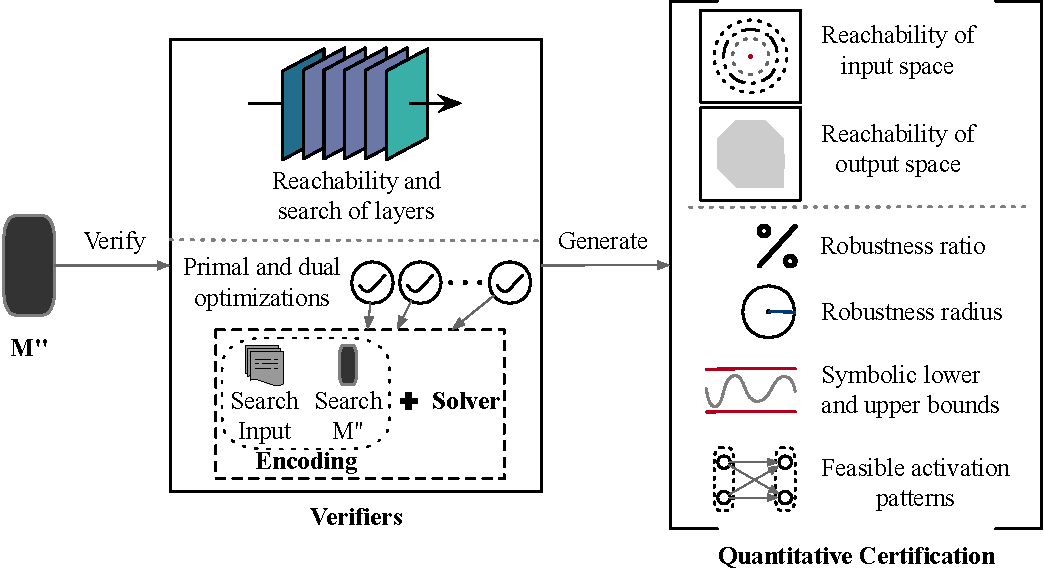
\includegraphics[scale=0.75]{fig/task4.pdf}
    \caption{Quantitative verification}
    \label{fig:task4}
\end{figure}

\textcolor{pink}{indicators of quantitative certification}

\textcolor{blue}{We will propose multiple quantitative verification approaches for generating a certification. The first category of approaches is the reachability of the input and output space through searching the network layers. More specifically, given an input constraint, the approaches will propagate the geometric sets layer by layer from the input layer to the output layer to get the reachable set. There is a comparison between the reachable set and the existing output constraint. The reachability will hold if contained; otherwise, the property is not held. The second category of approaches is the primal and dual optimizations through encoding and solving the input space and model. More specifically, the model will be encoded to model counting constraints and verified through abstract symbolic execution and model generation at symbolic execution tree nodes. The quantitative robustness certification consists of the reachability of input and output space, robustness ratio, robustness radius, lower and upper bounds, and feasible activation patterns. The quantitative verification processes are in Figure~\ref{fig:task4}.}

\textcolor{blue}{\textbf{Input and output space reachability}.  The reachability of input space and output space are denoted as $\mathcal{R}_{input}(\mathcal{X})$ and $\mathcal{R}_{output}(\mathcal{Y}, \mathrm{M}'')$. $\mathcal{X}$ is the input dataset with \emph{m} records and \emph{n} dimensions. $d_{i,j}$ is the value in $\mathcal{X}$. $\mathcal{Y}$ is the expected output set of $\mathcal{X}$ at the same row. }
\begin{equation}
\mathcal{R}_{input}(\mathcal{X})=\left[ (\min_{\genfrac{}{}{0pt}{2}{i=0,\dotsm,n-1} {0}} d_{i, 0},\max_{\genfrac {}{}{0pt}{2}{i=0,\dotsm, n-1 }{0}} d_{i, 0}),\dotsm, (\min_{\genfrac{}{}{0pt}{2}{i=0,\dotsm, n-1}{j-1}}d_{i, j-1},\max_{\genfrac {}{}{0pt}{2}{i=0,\dotsm, n-1}{j-1}} d_{i, j-1}) \right] s.t. \mathcal{R}_{output}(\mathcal{D}_{in}, \mathcal{N}) \subset \mathcal{D}_{out}
\end{equation}


\textcolor{blue}{\textbf{Robustness ratio}. For a neural network $\mathcal{N}$, an input $\mathcal{X}=\langle x_0, \dotsm, x_{n-1} \rangle$, a perturbation limit $\mathcal{P}^{lim}= \langle p^{lim}_{0}, \dotsm, p^{lim}_{n-1} \rangle$ denoting the perturbation limit value per feature, $S_{Area}$ denoting all perturbed inputs within $\mathcal{P}^{lim}$, $S_{RobustArea}$ denoting all perturbed inputs within the limit that the output of $\mathcal{N}$ does not change, $\bar{X}$ denoting the set of $x_i\in \mathcal{X}$ within the conditions.  The robustness ratio $R_{r}$ calculates as follows.}

\begin{equation}   R_{r}(\mathcal{N},\mathcal{X},\mathcal{P}^{lim})=\frac{\lvert S_{RobustArea}\rvert}{\lvert S_{Area}\rvert}
\end{equation}
\begin{equation}
    S_{RobustArea}=\lbrace\bar{X}|\:arg\:max\:\mathcal{N}(\bar{X}) =arg\:max\:\mathcal{N}(\mathcal{X})\:\:\wedge\:\: x_i-p^{lim}_i\leqslant \bar{x_i}\leqslant x_i + p^{lim}_i\rbrace
\end{equation}
\begin{equation}
    S_{Area}=\lbrace\bar{X}|\:\: x_i-p^{lim}_i\leqslant \bar{x_i}\leqslant x_i + p^{lim}_i\rbrace
\end{equation}

\textcolor{blue}{\textbf{Robustness radius.} Given a network $\mathcal{N}$, an input \emph{x}, a norm $\mathtt{p}$, and a distance $d$, the maximum robustness radius ($MRR$) is to compute the minimum distance from input \emph{x} to a counterexample \emph{x'}.}
\begin{equation}
        MRR(\mathcal{N},x,\mathtt{p},d)=\max_{d}\left\{ \left\| x-x' \right\|_\mathbf{p} < d \ |\  Robust({\mathcal{N}, x',\mathtt{p},d}) == \texttt{True},\  \mathcal{N}(x) = \mathcal{N}(x')\right\}
\end{equation}

\textcolor{blue}{\textbf{Lower and upper bounds.} The lower and upper bounds on $v_{i,j}$ which is the value of node \emph{j} on layer \emph{i} before activation function $\sigma$ are denoted as $l_{i,j}$ and $u_{i,j}$. $l_i$ and $u_i$ denote the lower and upper bounds of \emph{i}th layer $v_i$. The lower and upper bounds on $\hat{v}_{i,j}$ which is the value of node \emph{j} on layer \emph{i} after activation function are denoted as $\hat{l}_{i,j}$ and $\hat{u}_{i,j}$. The lower and upper bounds of \emph{i} layer before activation function are $L_i=\max l_{i,j}$ and $U_i=\max u_{i,j}$. $\hat{L}_i=\min \hat{l}_{i,j}$ and $\hat{U}_i=\max\hat{u}_{i,j}$ are the lower and upper bounds of \emph{i} layer after the activation function. }
\begin{equation}
    l_{i,j}= \min_{v_{i-1}\in [ l_{i-1}, u_{i-1} ]  } w_{i,j} v_{i-1} +b_{i,j}
\end{equation}
\begin{equation}
    u_{i,j}= \max_{v_{i-1}\in \left [ l_{i-1}, u_{i-1} \right ]  } w_{i,j} v_{i-1} +b_{i,j}
\end{equation}
\begin{equation}
    \hat{l}_{i,j}= \min_{v_{i,j}\in \left [ l_{i,j}, u_{i,j} \right ]  } \sigma_{i,j} (v_{i,j})=\sigma_{i,j}(l_{i,j})
\end{equation}
\begin{equation}
    \hat{u}_{i,j}= \max_{v_{i,j}\in \left [ l_{i,j}, u_{i,j} \right ]  } \sigma_{i,j} (v_{i,j})=\sigma_{i,j}(u_{i,j})
\end{equation}

\textcolor{blue}{\textbf{Feasible activation patterns}.}

\textcolor{pink}{new: handling more activation functions}

\textcolor{blue}{ Current verification approaches handling piece-wise linear activation functions mainly consider ReLU functions. A few consider Sigmoid and Softmax. The verification approaches in our project will handle other activation functions such as Exponential Linear Units (ELUs)~\cite{clevert2015fast} speeding up comparing ReLU on ImageNet and Gaussian Error Linear Unit(GELU)~\cite{hendrycks2016gaussian} outperforming in CV and NLP tasks. }

\textcolor{pink}{new: handling RNN}

\textcolor{blue}{The input of task 4 will have feedforward neural networks and recurrent neural networks (RNN). Current research works on feedforward neural networks. We will propose a method to transform RNNs into feedforward neural networks to adapt to verification approaches.}




\begin{comment}
\begin{figure}[t]
    \centering
    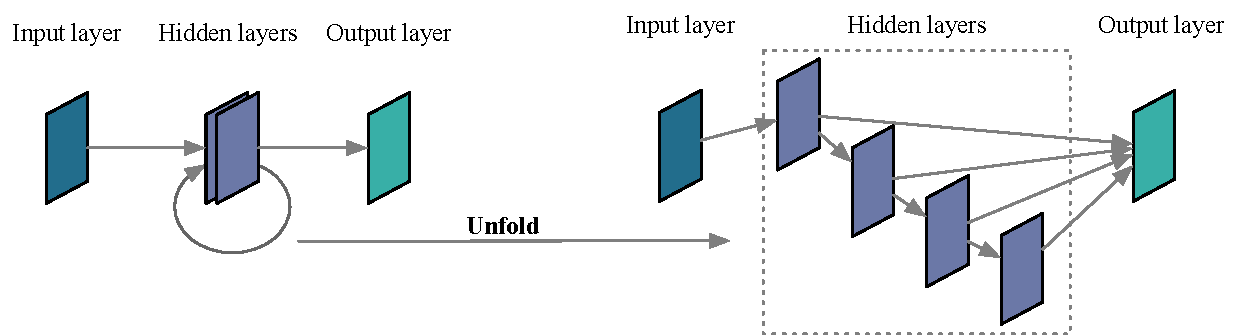
\includegraphics[scale=0.65]{fig/unfoldRNN.pdf}
    \caption{Unfold RNN to feedforward neural network}
    \label{fig:unfold}
\end{figure}
\textcolor{green}{balance between accuracy and scalability}

To calculate the decision boundary (between malicious and benign), we need only apply what ever learner we are uses to its own training data. This will assign classifications (malicious or benign) to every training example. Then, for each example:
\bi
\item Find its nearest neighbor with a different classification;
\item Sort every example by its distance to its nearest unlike neighbor;
\item Look a the top (say) 100 pairs.
\ei
Then, to see it two learners have the same boundary, compute the Jaccard index (intersection divided by overlap) of their top 100 pairs.
  



    \subsubsection{Trade-offs and Risks}\label{r1}
This part is the foundation of the following learning strategies. 
However, the following research will be delayed if too much time is spent on this task. 
Hence, we will conduct some simple studies to sort these factors and continue the studies following this ranking. 
Then, if this task takes too long, we might analyze the current results and move to \textbf{GOAL2} on these results.
\end{comment}
